\documentclass[12pt,aspectratio=169]{beamer}
\usetheme{metropolis}
\setbeamersize{text margin left=.5cm,text margin right=.5cm}
\usepackage[lf]{carlito}
\usepackage{siunitx}
\usepackage{tikz}
\usepackage{mathpazo}
\usepackage{bm}
\usepackage{mathtools}
\usepackage[ISO]{diffcoeff}
\diffdef{}{ op-symbol=\mathsf{d} }
\usepackage{xcolor,colortbl}

\setmonofont{Ubuntu Mono}
\setlength{\parskip}{0pt}
\renewcommand{\baselinestretch}{1}

\sisetup{
  inter-unit-product=\cdot,
  per-mode=symbol
}

\tikzset{
  >=latex
}

%\newcommand{\iii}{\hat{\bm\imath}}
%\newcommand{\jjj}{\hat{\bm\jmath}}
%\newcommand{\kkk}{\hat{\bm k}}


\title{Class 19: Magnetism, Part 3}
\subtitle{Advanced Placement Physics C}
\author[TML]{Dr.\ Timothy Leung}
\institute{Olympiads School}
\date{Updated: Summer 2022}

\newcommand{\pic}[2]{
  \includegraphics[width=#1\textwidth]{#2}
}
\newcommand{\eq}[2]{
  \vspace{#1}{\Large
    \begin{displaymath}
      #2
    \end{displaymath}
  }
}
%\newcommand{\iii}{\ensuremath\hat{\bm{\imath}}}
%\newcommand{\jjj}{\ensuremath\hat{\bm{\jmath}}}
%\newcommand{\kkk}{\ensuremath\hat{\bm{k}}}
\newcommand{\iii}{\ensuremath\hat\imath}
\newcommand{\jjj}{\ensuremath\hat\jmath}
\newcommand{\kkk}{\ensuremath\hat k}



\begin{document}

\begin{frame}
  \maketitle
\end{frame}


\section{Additional Notes on Motional EMF}

\begin{frame}{Motional EMF}
  \begin{columns}
    \column{.45\textwidth}
    \centering
    \begin{tikzpicture}
      \foreach \x in {1,...,6}
      \foreach \y in {0,...,3} \node[cyan] at (\x,\y) {$\times$};
      \draw[line width=.6mm](1.3,.5)--(6,.5);
      \draw[line width=.6mm](1.3,2.5)--(6,2.5);
      \draw[line width=1.7mm,red!60!black](4.5,.1)--(4.5,3.3);
      \draw[thick,<->](2.8,.53)--(2.8,2.47)node[midway,fill=black!2]{$\ell$};
      \draw[thick,|<->](1.3,.2)--(4.5,.2) node[pos=.42,fill=black!2]{$x$};
      \draw[very thick,->](4,3.5)--(5,3.5) node[right]{$\vec v$};
      %\draw[very thick,->,orange](4.58,1.5)--(5.5,1.5) node[right]{$\vec F_a$};
      \draw[thick](1.3,.47) to[R=$R$] (1.3,2.53);
      \node[cyan] at (1.5,3.2) {$\vec B_\text{in}$};
    \end{tikzpicture}
    
    \column{.55\textwidth}
    When sliding the rod to the right with constant velocity $\vec v$, magnetic
    flux $\Phi_m$ through the circuit loop is:

    \eq{-.2in}{
      \Phi_m=B{\color{magenta}A}=B{\color{magenta}\ell x}
    }

    \vspace{-.1in}Induced emf is:
    
    \eq{-.1in}{
      |\mathcal E|
      =\left|\frac{\Delta\Phi_m}{\Delta t}\right|
      =\frac{B\ell{\color{violet}x}}{\color{violet}\Delta t}
      =B\ell{\color{violet}v}
    }

    The induced current through the circuit can easily be caclulated using
    Ohm's law:

    \eq{-.15in}{
      I=\frac{\mathcal E}R=\frac{B\ell v}R
    }
  \end{columns}
\end{frame}



\begin{frame}{Induced Current from Motional EMF}
  \begin{columns}
    \column{.45\textwidth}
    \centering
    \begin{tikzpicture}
      \foreach \x in {1,...,6}
      \foreach \y in {0,...,3} \node[cyan] at (\x,\y) {$\bm\times$};
      \draw[lightgray,line width=.6mm](1.3,.5)--(6,.5);
      \draw[lightgray,line width=.6mm](1.3,2.5)--(6,2.5);
      \draw[line width=1.7mm,lightgray](4.5,.1)--(4.5,3.3);
      \draw[very thick,->](4,3.5)--(5,3.5) node[right]{$\vec v$};
      %\draw[very thick,->](4.55,1.5)--(5.5,1.5) node[right]{$F_a$};
      \draw[thick] (1.3,.47) to[R=$R$] (1.3,2.53);
      \node[cyan] at (1.5,3.2) {$\vec B_\text{in}$};
      \draw[violet,ultra thick,->](4.5,.7)--(4.5,2.2) node[above]{$I$};
      \draw[violet,ultra thick,->](4,2.5)--(2,2.5) node[midway,above]{$I$};
      \draw[violet,ultra thick,->](2,.5)--(4,.5) node[midway,above]{$I$};
    \end{tikzpicture}

    \column{.55\textwidth}

    Induced current $I$ runs counter-clockwise, because (by Lenz's law) it must
    produce a magnetic field that \emph{oppose the increase in magnetic flux}.
    The power dissipated by the (ohmic) resistor is:

    \eq{-.2in}{
      P=I^2R=\left[\frac{B\ell v}R\right]^2R=\frac{B^2\ell^2v^2}R
    }

    \textbf{But where did the energy come from?}
  \end{columns}
\end{frame}



\begin{frame}{Magnetic Force on Induced Current}
  \begin{columns}
    \column{.45\textwidth}
    \centering
    \begin{tikzpicture}
      \foreach \x in {1,...,6}
      \foreach \y in {0,...,3} \node[cyan] at (\x,\y) {$\bm\times$};
      \draw[line width=.6mm](1.3,.5)--(6,.5);
      \draw[line width=.6mm](1.3,2.5)--(6,2.5);
      \draw[line width=1.7mm,red!70!black](4.5,.1)--(4.5,3.3);
      \draw[thick,<->](2.8,.53)--(2.8,2.47)node[midway,fill=black!2]{$\ell$};
      \draw[very thick,->](4,3.5)--(5,3.5) node[right]{$\vec v$};
      \draw[very thick,->,orange](4.58,1.5)--(5.5,1.5) node[right]{$\vec F_a$};
      \draw[thick](1.3,.47) to[R=$R$] (1.3,2.53);
      \node[cyan] at (1.5,3.2) {$\vec B_\text{in}$};
      \foreach \yy in {.6,.9,...,2.5}
      \draw[orange,very thick,->] (4.42,\yy)--(3.8,\yy);
      \node[left,orange] at (3.9,1.5){$\vec F_m$};
      \draw[black!10,ultra thick,->](4.5,.7)--(4.5,2.2) node[above]{$I$};
    \end{tikzpicture}
    
    \column{.55\textwidth}
    The induced current $I$ in the rod is moving in a magnetic field, therefore
    it will experience a magnetic force $\vec F_m$ with a magnitude of:

    \eq{-.15in}{
      F_m=I\ell B = \left[\frac{B\ell v}R\right]\ell B
      =\frac{B^2\ell^2v}R
    }

    For a constant $\vec v$, an external force of $F_a=F_m$ must be applied,
    (see figure left). The power generated by the applied force is:

    \eq{-.2in}{
      P = F_av=F_mv=\left[\frac{B^2\ell^2v}R\right]v=\frac{B^2\ell^2v^2}R
    }
  \end{columns}
\end{frame}



\begin{frame}{Energy Conservation}
  \begin{columns}
    \column{.45\textwidth}
    \centering
    \begin{tikzpicture}
      \foreach \x in {1,...,6}
      \foreach \y in {0,...,3} \node[cyan] at (\x,\y) {$\bm\times$};
      \draw[line width=.6mm](1.3,.5)--(6,.5);
      \draw[line width=.6mm](1.3,2.5)--(6,2.5);
      \draw[line width=1.7mm,red!70!black](4.5,.1)--(4.5,3.3);
      \draw[very thick,->](4,3.5)--(5,3.5) node[right]{$\vec v$};
      \draw[very thick,->,orange](4.58,1.5)--(5.5,1.5) node[right]{$\vec F_a$};
      \draw[thick](1.3,.47) to[R=$R$] (1.3,2.53);
      \node[cyan] at (1.5,3.2) {$\vec B_\text{in}$};
    \end{tikzpicture}
        
    \column{.55\textwidth}
    The power generated by the applied force is equal to the power dissipated
    by the resistor that we have calculated:

    \eq{-.1in}{
      P = \frac{B^2\ell^2v^2}R
    }

    Therefore, the energy in the circuit comes from the positive work done by
    the applied force, and very importantly, our calculations confirm the law of
    conservation of energy.
  \end{columns}
\end{frame}



\section{Assymmetry in Faraday's Law}

\begin{frame}{A Coil Moving Through a Magnetic Field}
  A loop of wire moves through a magnetic field $\vec B$ into the page with
  velocity $\vec v$. From Faraday's law, when the wire moves \emph{into} the
  magnetic field, and when it moves \emph{out} of the field, magnetic flux
  $\Phi_m$ changes, creating an electromotive force $\mathcal E$:

  \eq{-.1in}{
    \boxed{ \mathcal E=-\diff{\Phi_m}t }
  }
  \begin{center}
    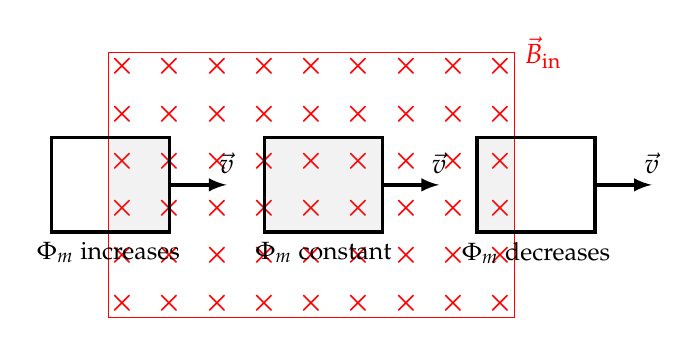
\begin{tikzpicture}[scale=.6]
      \draw[red](-.3,-.3) rectangle(8.3,5.3) node[right]{$\vec B_\text{in}$};
      \foreach\x in {0,1,...,8}{
        \foreach\y in {0,1,...,5} \node[red] at (\x,\y) {$\bm\times$};
      }
      
      \fill[gray,opacity=.1](-.3,1.5) rectangle(1,3.5);
      \draw[very thick](-1.5,1.5) rectangle(1,3.5);
      \draw[very thick,->](1,2.5)--(2.2,2.5) node[above]{$\vec v$};
      \node[below] at (-.3,1.5) {\small $\Phi_m$ increases};

      \uncover<2->{
        \fill[gray,opacity=.1](3,1.5) rectangle(5.5,3.5);
        \draw[very thick](3,1.5) rectangle(5.5,3.5);
        \draw[very thick,->](5.5,2.5)--(6.7,2.5) node[above]{$\vec v$};
        \node[below] at (4.25,1.5) {\small $\Phi_m$ constant};
      }
      \uncover<3->{
        \fill[gray,opacity=.1](7.5,1.5) rectangle(8.3,3.5);
        \draw[very thick](7.5,1.5) rectangle(10,3.5);
        \draw[very thick,->](10,2.5)--(11.2,2.5) node[above]{$\vec v$};
        \node[below] at (8.75,1.5) {\small $\Phi_m$ decreases};
      }
    \end{tikzpicture}
  \end{center}

  \vspace{-.1in}

\end{frame}



\begin{frame}{Coil Moving Through a Magnetic Field}
  For an observer in the same frame of reference as the magnetic field, the
  reason is obvious. The charges\footnote{presumably positive, but it doesn't
    really matter} inside the wire experience a \emph{magnetic force} as they
  move through the magnetic field, creating an \emph{emf}, and an electric
  current. This is called \textbf{motional EMF}.
  \begin{center}
    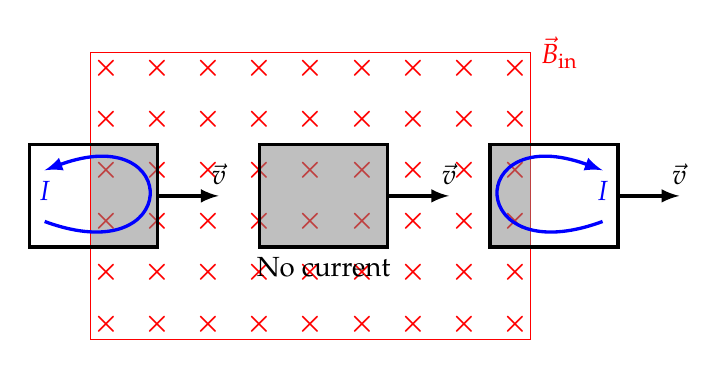
\begin{tikzpicture}[scale=.65]
      \draw[red](-.3,-.3) rectangle(8.3,5.3) node[right]{$\vec B_\text{in}$};
      \foreach\x in {0,1,...,8}{
        \foreach\y in {0,1,...,5} \node[red] at (\x,\y) {$\bm\times$};
      }
      
      \fill[gray,opacity=.5](-.3,1.5) rectangle(1,3.5);
      \draw[very thick](-1.5,1.5) rectangle(1,3.5);
      \draw[very thick,->](1,2.5)--(2.2,2.5) node[above]{$\vec v$};
      \draw[very thick,->,blue](-1.2,2)..controls(1.5,1) and (1.5,4)..(-1.2,3)
      node[below]{$I$};

      \uncover<2->{
        \fill[gray,opacity=.5](3,1.5) rectangle(5.5,3.5);
        \draw[very thick](3,1.5) rectangle(5.5,3.5);
        \draw[very thick,->](5.5,2.5)--(6.7,2.5) node[above]{$\vec v$};
        \node[below] at (4.25,1.5) {No current};
      }
      \uncover<3->{
        \fill[gray,opacity=.5](7.5,1.5) rectangle(8.3,3.5);
        \draw[very thick](7.5,1.5) rectangle(10,3.5);
        \draw[very thick,->](10,2.5)--(11.2,2.5) node[above]{$\vec v$};
        \draw[very thick,->,blue](9.7,2)..controls(7,1) and (7,4)..(9.7,3)
        node[below]{$I$};
      }
    \end{tikzpicture}
  \end{center}
  \vspace{.2in}
\end{frame}




\begin{frame}{Magnetic Field Moving Past a Coil of Wire}
  For an observer in the same frame of reference as the wire, the reason is
  also obvious. As the magnetic field moves, the magnetic flux changes, and an
  \emph{electric field} is created in the wire. A current is created because
  the charges inside the wire experience an \emph{electric force}.
  \begin{center}
    \vspace{-.15in}
    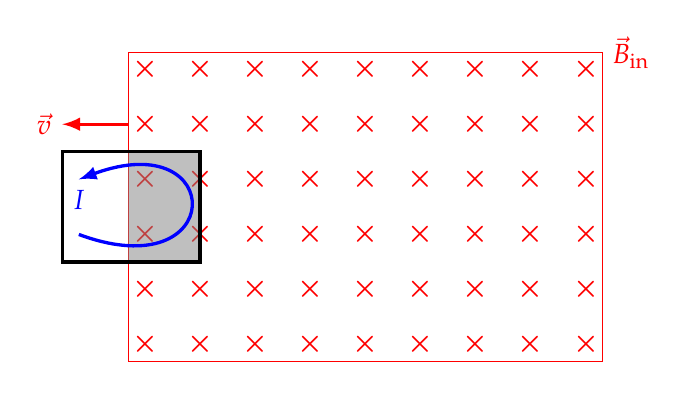
\begin{tikzpicture}[scale=.7]
      \draw[red](-.3,-.3) rectangle(8.3,5.3) node[right]{$\vec B_\text{in}$};
      \draw[red,very thick,->](-.3,4)--(-1.5,4) node[left]{$\vec v$};
      \foreach\x in {0,1,...,8}{
        \foreach\y in {0,1,...,5} \node[red] at (\x,\y) {$\bm\times$};
      }
      
      \fill[gray,opacity=.5](-.3,1.5) rectangle(1,3.5);
      \draw[very thick](-1.5,1.5) rectangle(1,3.5);
      \draw[very thick,->,blue](-1.2,2)..controls(1.5,1) and (1.5,4)..(-1.2,3)
      node[below]{$I$};
    \end{tikzpicture}
  \end{center}
\end{frame}


\begin{frame}{Assymmetry in Faraday's Law}
  Both observers obtain the same result (same $\mathcal E$ and same current $I$
  in the wire), however they cannot agree on the \emph{reason}. The bottom line:
  \begin{itemize}
  \item Faraday's law is the same in both frames of reference (principle of
    relativity)
  \item Magnetic force is just the electric force when viewed from a different
    frame of reference
  \item This ``asymmetry'' in Faraday's law led to the discovery of the theory
    of special relativity
  \end{itemize}
\end{frame}
\end{document}
